\chapter{Khảo sát}
\label{Chapter2}

\emph{Chương này giới thiệu về một số hệ thống tương tự với hệ thống chatbot cũng như một số thuật toán xử lí hiểu ngôn ngữ tự nhiên.}

\section{Chatbot}
\subsection{Chatbot là gì?}

Chatbot - hay còn được gọi là chatterbot - là một ứng dụng phần mềm được sử dụng để thực hiện một cuộc trò chuyện trực tuyến thông qua văn bản hoặc chuyển văn bản thành giọng nói, thay cho việc cung cấp liên hệ trực tiếp với một nhân viên trực tiếp. Trợ lý ảo chatbot đang ngày càng được sử dụng để xử lý các tác vụ đơn giản, tra cứu trong cả môi trường doanh nghiệp với người tiêu dùng và doanh nghiệp với doanh nghiệp.

Chatbot có thể có nhiều mức độ phức tạp khác nhau, không trạng thái hoặc trạng thái. Một chatbot không trạng thái tiếp cận mỗi cuộc trò chuyện như thể nó đang tương tác với một người dùng mới. Ngược lại, một chatbot trạng thái có thể xem xét các tương tác trong quá khứ và định khung các phản hồi mới theo ngữ cảnh\cite{chat-bot}.

Chatbot có thể được phân chia thành các loại sau đây:
\begin{itemize}
    \item Chatbot có kịch bản hoặc trả lời nhanh - Đây là những chatbot cơ bản nhất; chúng hoạt động như một cây quyết định phân cấp. Các bot này tương tác với người dùng thông qua một tập hợp các câu hỏi được xác định trước sẽ tiến triển cho đến khi chatbot trả lời câu hỏi của người dùng. Tương tự như chatbot này là chatbot dựa trên menu yêu cầu người dùng thực hiện các lựa chọn từ danh sách hoặc menu được xác định trước để cung cấp cho bot hiểu sâu hơn về những gì khách hàng đang tìm kiếm.

    \item Chatbot dựa trên nhận dạng từ khóa - Những chatbot này phức tạp hơn một chút; họ cố gắng lắng nghe những gì người dùng nhập và phản hồi tương ứng bằng cách sử dụng các từ khóa chọn được từ phản hồi của khách hàng. Các từ khóa có thể tùy chỉnh và AI được kết hợp trong bot này để cung cấp phản hồi thích hợp cho người dùng. Thật không may, những chatbot này phải vật lộn khi phải đối mặt với việc sử dụng từ khóa lặp đi lặp lại hoặc các câu hỏi thừa.

    \item Chatbot kết hợp - Những chatbot này kết hợp các yếu tố của bot dựa trên menu và nhận dạng từ khóa. Người dùng có thể chọn để câu hỏi của họ được trả lời trực tiếp, nhưng cũng có thể truy cập menu của chatbot để thực hiện lựa chọn nếu quá trình nhận dạng từ khóa tạo ra kết quả không hiệu quả.

    \item Chatbot theo ngữ cảnh - Những chatbot này phức tạp hơn những chatbot được liệt kê ở trên và yêu cầu tập trung vào dữ liệu. Họ sử dụng ML và AI để ghi nhớ các cuộc trò chuyện và tương tác với người dùng, sau đó sử dụng những ký ức này để phát triển và cải thiện theo thời gian. Thay vì dựa vào từ khóa, những bot này sử dụng những gì khách hàng yêu cầu và cách họ yêu cầu để đưa ra câu trả lời và tự cải thiện.

    \item Chatbot hỗ trợ giọng nói - Loại chatbot này là tương lai của công nghệ chatbot. Các chatbot hỗ trợ giọng nói sử dụng đối thoại bằng giọng nói từ người dùng làm dữ liệu đầu vào. Chúng có thể được tạo bằng cách sử dụng văn bản thành giọng nói (\ac{tts}) và giao diện chương trình ứng dụng nhận dạng giọng nói (\ac{api}) \cite{chat-bot}.

\end{itemize}
Ưu điểm của chatbot:
\begin{itemize}
    \item Cung cấp dịch vụ khách hàng nhanh chóng hơn:
          \begin{itemize}
              \item[--] Phần mềm này hỗ trợ doanh nghiệp cung cấp dịch vụ khách hàng 24 giờ/ngày, bất kể cuối tuần hay nghỉ lễ.
              \item[--] Khi khách hàng trực tuyến có thắc mắc, họ chỉ cần hỏi trong chatbot trên trang web của chúng ta mà không cần phải chờ đợi lâu để có câu trả lời. Bởi câu trả lời chỉ là một vài tổ hợp được lập trình sẵn.
          \end{itemize}
    \item Làm tăng sự hài lòng của khách hàng:
          \begin{itemize}
              \item[--] Khi khách hàng nhận được câu trả lời thỏa đáng với dịch vụ nhanh chóng nhờ chatbot, họ sẽ cảm thấy hài lòng hơn và tiếp tục mua sản phẩm của chúng ta.
          \end{itemize}
    \item Giảm chi phí lao động:
          \begin{itemize}
              \item[--] Chatbot giúp bạn giữ chi phí kinh doanh thấp bởi số tiền bạn đầu tư vào chatbot ít hơn số tiền bạn phải trả cho nhân viên.
              \item[--] Bằng cách này, bạn thực sự tiết kiệm được rất nhiều tiền thay vì việc duy trì một trung tâm hỗ trợ khách hàng. Tính năng này sẽ giúp bạn tiết kiệm tài chính, tránh những rắc rối trong quản lý nhân sự, và tiết kiệm thời gian để làm những việc cần thiết khác.
          \end{itemize}
    \item Nhiều mục đích sử dụng:
          \begin{itemize}
              \item[--] Bạn có thể sử dụng chatbot trong nhiều mảng, ví dụ như nhận đơn đặt hàng của khách, dịch vụ khách hàng và quảng cáo sản phẩm.
          \end{itemize}
\end{itemize}
\subsection{Kiến trúc cơ bản của Chatbot}
\begin{figure}[htp]
    \centering
    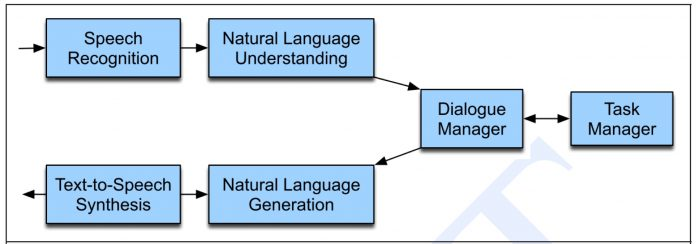
\includegraphics[width=10cm]{images/k.jpg}
    \caption{Kiến trúc cơ bản của một hệ thống giao tiếp tự động}
    \label{fig:k}
\end{figure}

Các hệ thống chatbot giao tiếp với con người bằng giọng nói (như Siri \footnote{Xem thêm về Siri tại đây:\url{https://www.apple.com/siri/}}) hoặc bằng văn bản (như các chatbot phát triển trên nền Facebook Messenger \footnote{Xem thêm về Facebook Messenger tại đây:\url{https://www.apple.com/siri/}})). Dù giao tiếp bằng hình thức nào, chatbot cũng cần phải hiểu văn bản để có thể đưa ra những câu trả lời phù hợp cho khách hàng. Thành phần đảm nhiệm công việc này trong hệ thống chatbot được gọi là \ac{nlu}, trong đó có rất nhiều các kỹ thuật xử lý ngôn ngữ tự nhiên (\ac{nlp}) được áp dụng.
\\
Hai thành phần liên quan đến xử lý ngôn ngữ tự nhiên không thể thiếu của một \ac{nlu} module là bộ phân loại ý định và nhận diện thực thể (\ac{ner}). Phân loại ý định giúp chatbot hiểu ý định của người dùng. Về mặt bản chất phân loại ý định chính là một bài toán phân loại câu với tập nhãn là các ý định có thể có của người dùng (đã được định nghĩa từ trước). \ac{ner} giúp chatbot trích xuất các thông tin trong yêu cầu/câu trả lời của người dùng. Các thông tin đó có thể là tên sản phẩm, địa chỉ, số điện thoại, số tài khoản của người dùng,… \ac{ner} là một bài toán gán nhãn chuỗi cơ bản: cho vào một câu đầu vào, trích xuất tất cả các thực thể định danh trong câu và phân loại chúng vào một trong các nhãn đã được định nghĩa từ trước.
\\
Một thành phần xử lý ngôn ngữ tự nhiên khác có thể được thêm vào chatbot là bộ quản lý hội thoại, bộ sinh ngôn ngữ (\ac{nlg}), và bộ phân tích cảm xúc. Một bộ quản lý hội thoại sẽ lưu trữ, phân tích và tận dụng ngữ cảnh cuộc hội thoại và giúp chatbot suy luận hành động tiếp theo trong khi \ac{nlg} giúp sinh câu trả lời đầy đủ, tự nhiên nhất bằng ngôn ngữ tự nhiên cho chatbot. Một bộ phân tích cảm xúc có thể cần bởi vì cùng một câu có thể mang nhiều nghĩa khác nhau trong các văn cảnh khác nhau, do đó có thể cần được trả lời theo các cách khác nhau phụ thuộc vào cảm xúc của người dùng.
\\
Bài luận này chủ yếu nghiên cứu về phát hiện ý định và trích xuất thực thể trong NLU module.

\section{Các hệ thống tương tự}

Hiện nay, việc xây dựng chatbot trong nhiều lĩnh vực như kinh doanh, y tế, giải trí,... khá là phát triển và đem lại được nhiều lợi ích lớn đối với người dùng. Trong lĩnh vực chỉ đường, chúng em nhận thấy rằng hiện chưa có chatbot nào được xây dựng, nhưng cũng có không ít các ứng dụng dùng để chỉ đường như Google Maps\cite{ggmaps},...

Google Maps là một dịch vụ bản đồ web được phát triển bởi Google. Nó cung cấp hình ảnh vệ tinh, chụp ảnh trên không, bản đồ đường phố, chế độ xem toàn cảnh tương tác 360° của đường phố, điều kiện giao thông thời gian thực và lập kế hoạch tuyến đường để đi bộ, xe hơi, xe đạp và máy bay hoặc giao thông công cộng. Năm 2020, Google Maps được sử dụng bởi hơn 1 tỷ người mỗi tháng trên thế giới.

Google Maps khởi đầu được thiết kế bởi hai anh em người Đan Mạch, tại công ty Where 2 Technologies có trụ sở tại Sydney. Lần đầu tiên nó được thiết kế để người dùng tải xuống riêng biệt, nhưng sau đó công ty đã trình bày ý tưởng về một sản phẩm hoàn toàn dựa trên Web cho ban quản lý của Google, thay đổi phương thức phân phối. Vào tháng 10 năm 2004, công ty được mua lại bởi Google - nơi nó chuyển thành ứng dụng web Google Maps. Sản phẩm hiện đã xuất hiện ở cả hai phiên bản web và mobile.

Google Map hiện giờ rất phố biến đối với người dùng và nó có rất nhiều tính năng về vị trí, trong đó có thể nói tính năng chỉ dẫn đường đi là vô cùng phổ biến với người dùng.

Tính năng chỉ đường của Google Maps cung cấp công cụ lập kế hoạch tuyến đường, cho phép người dùng tìm chỉ đường khả dụng thông qua lái xe, giao thông công cộng, đi bộ hoặc đi xe đạp.

Ứng dụng Google Maps trên điện thoại cũng tích hợp sử dụng thu âm, chuyển giọng nói thành văn bản khi nhập điểm bắt đầu và điểm kết thúc để người dùng có thể dễ nhập điểm đầu và cuối.

\begin{figure}[H]
    \centering
    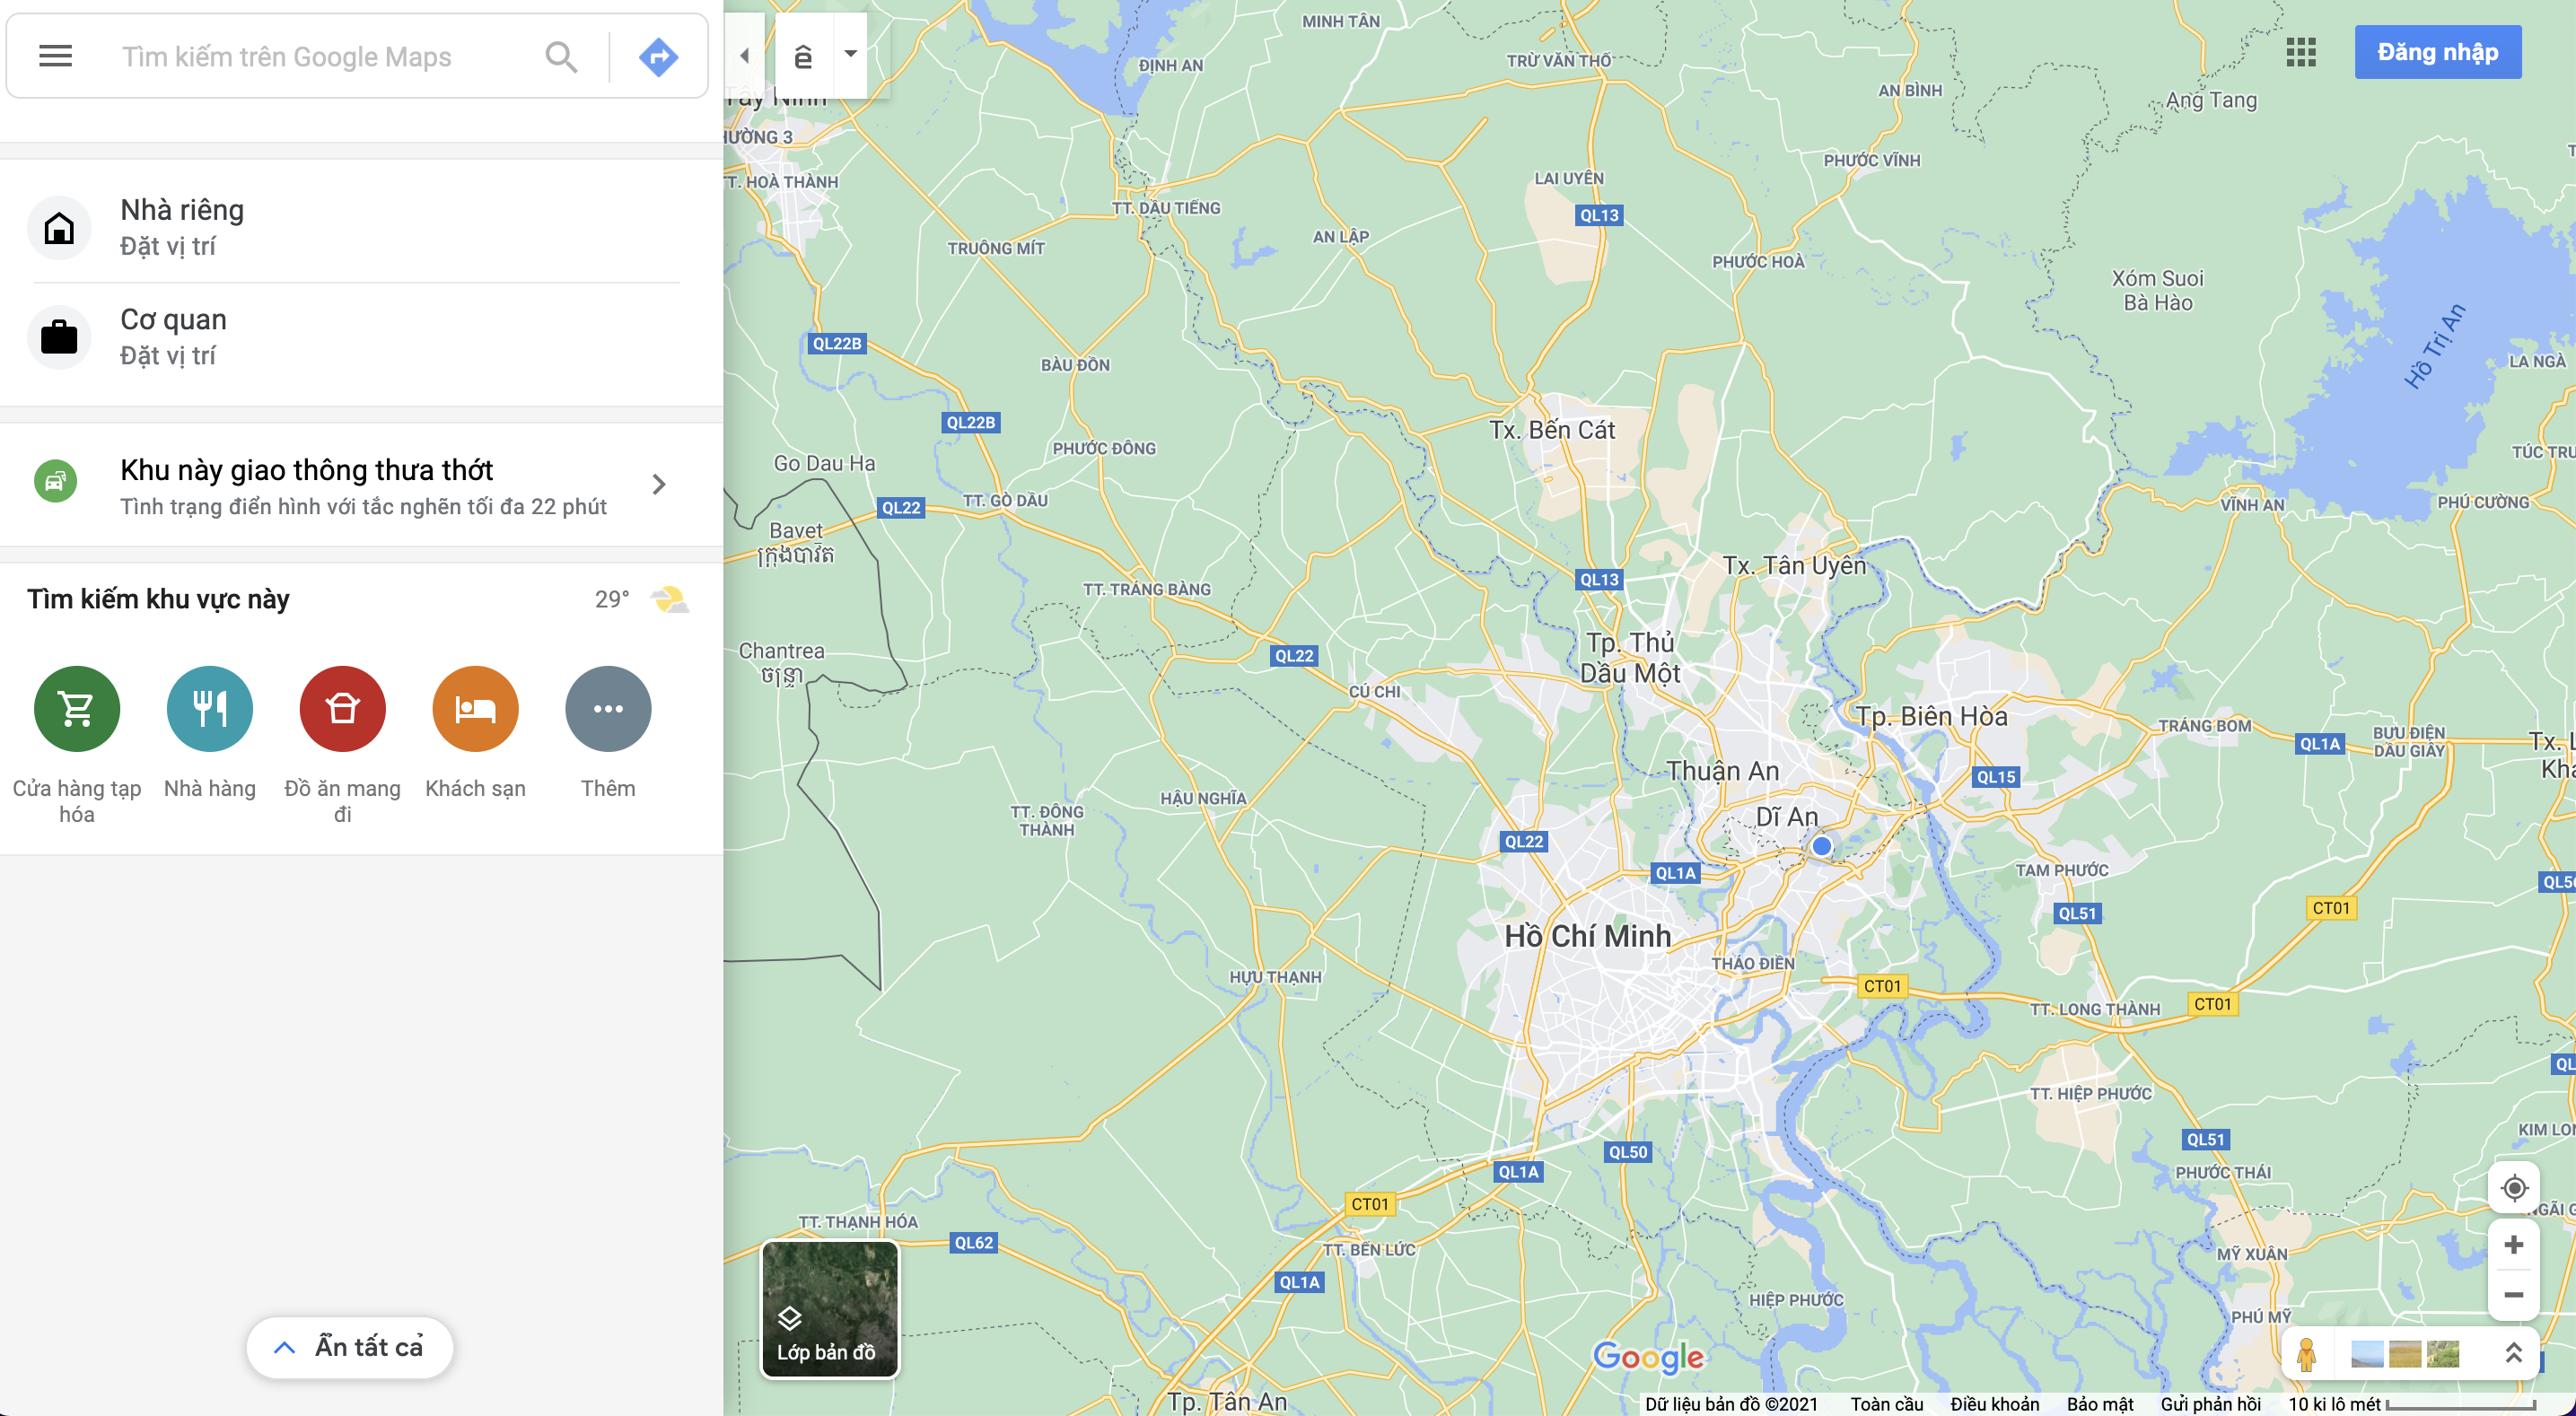
\includegraphics[width=10cm]{images/HomePage-GoogleMaps.png}
    \caption{Trang chủ Google Maps}
    \label{fig:homepage-ggmaps}
\end{figure}

Android Auto là một ứng dụng di động được phát triển bởi Google nhằm đưa các tính năng từ một thiết bị Android (ví dụ như điện thoại thông minh) lên hệ thống bảng thông báo và giải trí tương thích trên xe hơi.

\begin{figure}[H]
    \centering
    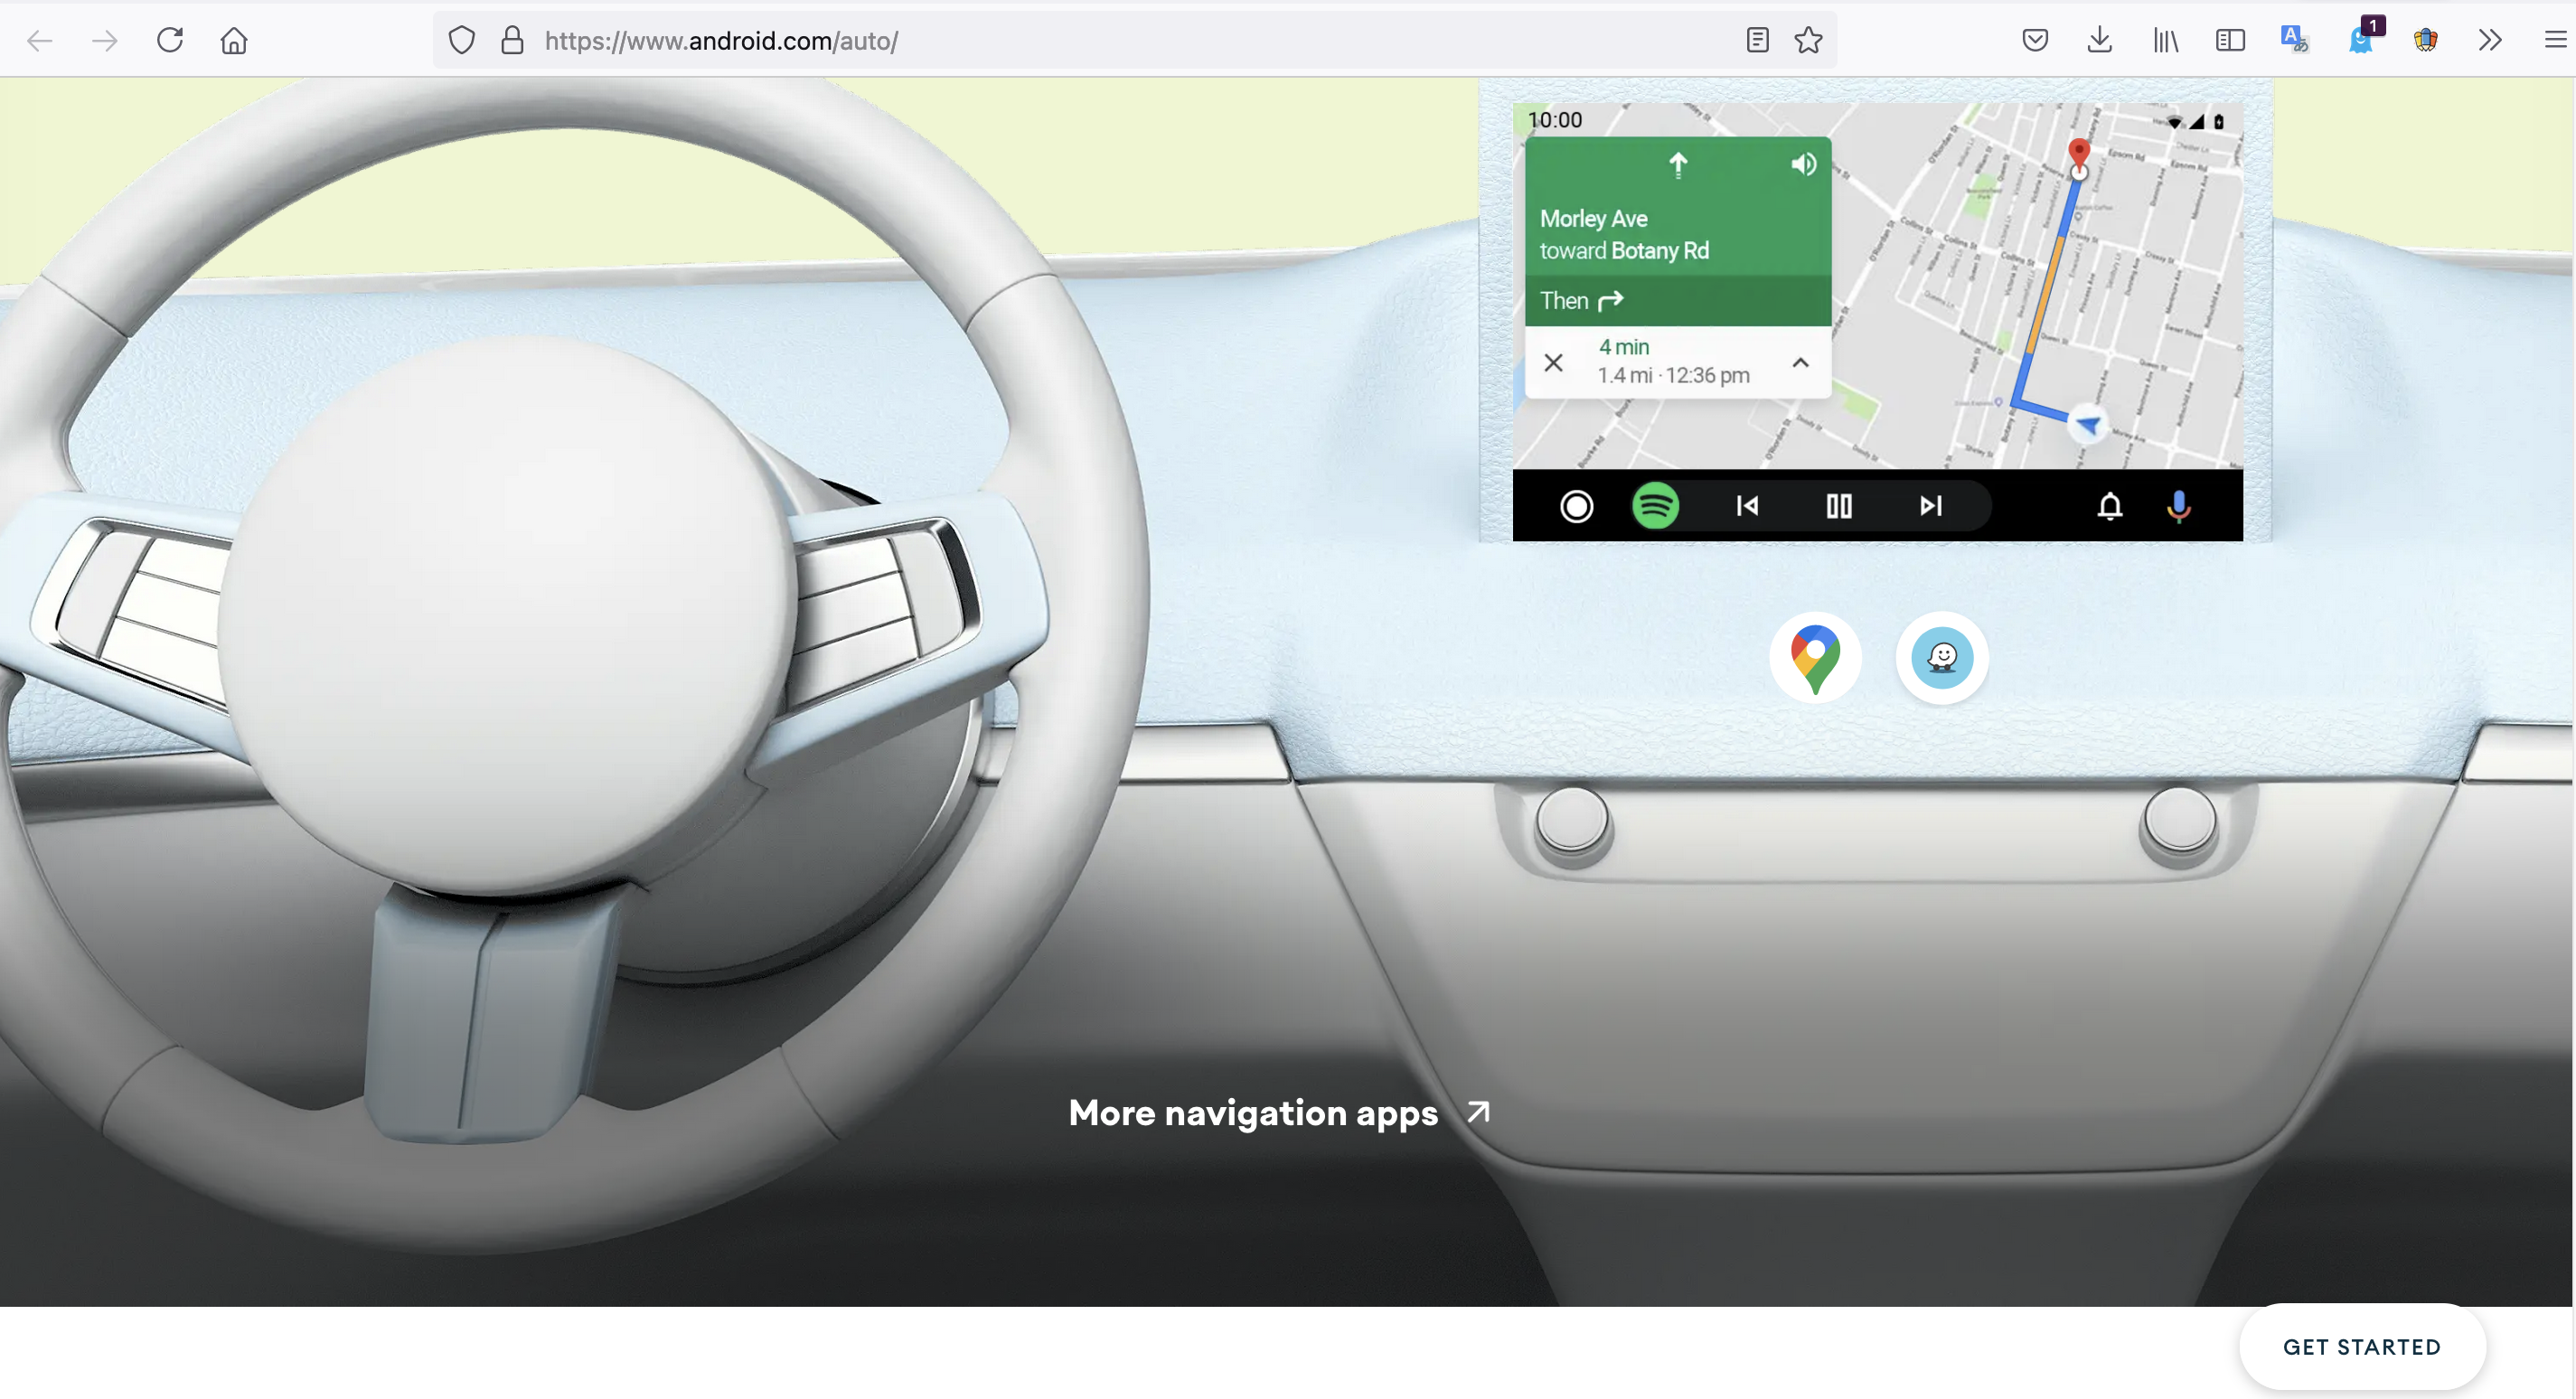
\includegraphics[width=10cm]{images/Android-Auto.png}
    \caption{Trang chủ Android Auto}
    \label{fig:homepage-android-auto}
\end{figure}

Kết nối điện thoại với màn hình ô tô — ứng dụng Android sẽ hiển thị trên màn hình hiển thị của xe. Nhấn để nhận chỉ đường lái xe hoặc nói chuyện để gửi tin nhắn. Thậm chí gọi điện thoại rảnh tay cho mẹ bạn. Android Auto được tạo ra để giúp bạn tập trung vào đường đi. Và vui vẻ trên đường đi. Chỉ cần cắm vào và đi.

\begin{figure}[H]
    \centering
    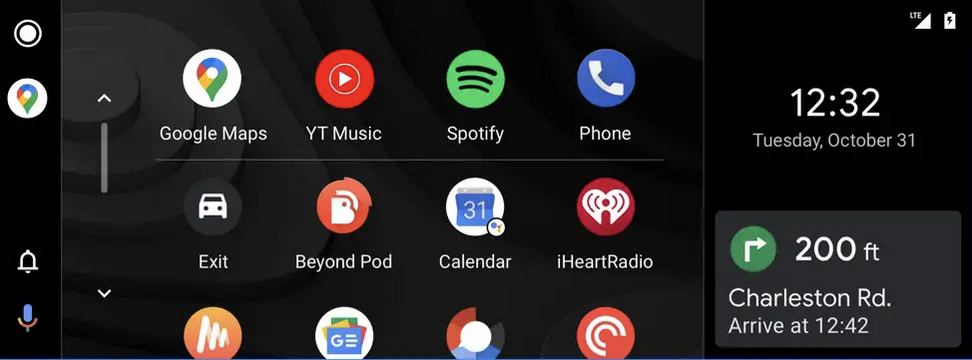
\includegraphics[width=10cm]{images/widescreen.png}
    \caption{Xem mọi thứ trên màn hình rộng.}
    \label{fig:homepage-widescreen-Android}
\end{figure}

Với mong muốn xây dựng một ứng dụng chatbot sử dụng trong lĩnh vực chỉ đường, chúng em xây dựng một ứng dụng tiếng Việt, trong đó có sử dụng giọng nói để tương tác với ứng dụng, hỏi đường chỉ bằng một câu nói dễ dàng, sử dụng được mọi lúc, một cách đơn giản mà không làm mất đi sự tập trung của người dùng khi lái xe.

\section{Các nền tảng hiểu ngôn ngữ tự nhiên}

Hiểu ngôn ngữ tự nhiên là thành phần rất quan trọng và không thể thiếu trong chatbot cũng như trợ lý ảo. Nó giúp chúng ta nhận diện ý định và các thực thể từ câu nói của người dùng.

Hiện nay có rất nhiều nền tảng cung cấp thành phần hiểu ngôn ngữ tự nhiên, trong số đó những dịch vụ NLU phổ biến nhất là: LUIS\footnote{\url{https://www.luis.ai/}}, Watson\footnote{\url{https://www.ibm.com/watson}}, DialogFlow\footnote{\url{https://cloud.google.com/dialogflow/docs/}}, Rasa\footnote{\url{https://rasa.com/}} và Snips\footnote{\url{https://snips.ai/}}.

\subsection{Các nền tảng NLU phổ biến}

\textbf{Dialogflow (Google):} Trước đây được gọi là Api.ai, gần đây nó đã đổi tên thành Dialogflow và nó là một nền tảng phát triển trợ lý văn bản ảo và nhanh chóng bổ sung khả năng nói. Framework này tạo ra chatbot thông qua giao diện người dùng dựa trên web hoàn chỉnh hoặc đối với các dự án phức tạp, sử dụng số lượng lớn các API thông qua Rest (cũng có nhiều SDK cho các ngôn ngữ lập trình khác nhau). Các ý định và thực thể khác nhau có thể được tạo ra bằng cách đưa ra các ví dụ. Nó hỗ trợ nhiều ngôn ngữ khác nhau.

\textbf{Watson (IBM):} Nền tảng này trở nên nổi tiếng vào năm 2011 vì nó đã giành chiến thắng trong một cuộc thi chống lại các nhà vô địch của con người của trò chơi nguy hiểm. Watson là một NLU framework hoàn chỉnh cho phép phát triển một chatbot bằng cách sử dụng một giao diện người dùng trên nền tảng web hoặc để khai thác các SDK khác nhau, để tạo một trợ lý ảo nhanh chóng và với các chương trình ngôn ngữ khác nhau. Nền tảng này dễ dàng tích hợp với nhiều dịch vụ truyền thông khác nhau và cung cấp hỗ trợ đầy đủ sang công nghệ Text-to-Speech và Speech-to-Text. Watson cho phép nhận ra ý định và thực thể, và một số mô hình liên quan đến chủ đề chung được cung cấp bởi nền tảng, trong khi đối với các miền cụ thể, người dùng phải tạo mô hình đưa ra một tập hợp các ví dụ khá nhỏ để đào tạo động cơ NLU.

\textbf{Luis (Microsoft):} Tương tự như các nền tảng trước, Luis là một dịch vụ dựa trên đám mây có sẵn thông qua giao diện web hoặc các yêu cầu API. Luis cung cấp nhiều mô hình miền được tạo sẵn bao gồm ý định, lời nói và thực thể, hơn nữa, nó cho phép xác định các mô hình tùy chỉnh. Việc quản lý luồng đối thoại dẫn đến phức tạp hơn cho các sản phẩm khác. Tuy nhiên, có thể xây dựng một trợ lý ảo hoàn chỉnh với các khả năng tương tự được cung cấp bởi các dịch vụ khác. Các công cụ khác nhau tạo điều kiện phát triển trợ lý ảo được hỗ trợ (chẳng hạn như hỗ trợ kiểm tra, phân tích văn bản thành lời nói và cảm xúc).

\textbf{Rasa NLU:} là một công cụ để hiểu những gì đang được nói trong các đoạn văn bản ngắn. Rasa NLU chủ yếu được sử dụng để xây dựng chatbot và ứng dụng thoại. Do là mã nguồn mở nên Rasa có thể được tùy chỉnh một cách dễ dàng để phù hợp với nhu cầu của người sử dụng.

\textbf{Snips NLU:}  là một công cụ hiểu ngôn ngữ tự nhiên cho phép phân tích cú pháp các câu được viết bằng ngôn ngữ tự nhiên và trích xuất thông tin có cấu trúc. Chỉ cần một ít dữ liệu đào tạo là có thể tạo ra một công cụ nhận dạng ý định mạnh mẽ. Snips NLU có thể được tùy chỉnh và hỗ trợ nhiều ngôn ngữ như tiếng Anh, tiếng Pháp, tiếng Đức, tiếng Ý, v.v...

\subsection{Yêu cầu lựa chọn}
Do sự tồn tại của nhiều dịch vụ NLU, việc lựa chọn ra một nền tảng để sử dụng cũng rất khó khăn. Nhóm em sẽ lựa chọn nền tảng NLU có hiệu năng cao để có thể đem lại kết quả tốt.

Nếu hiệu năng giữa các nền tảng thương mại và nền tảng mã nguồn mở không có sự chênh lệch nhiều, nhóm sẽ ưu tiên lựa chọn nền tảng NLU mã nguồn mở do những lợi ích sau:
\begin{itemize}
    \item[--] Chi phí:  tốn rất ít hoặc không có chi phí trả trước cho mã nguồn mở. chúng ta chỉ cần tải mã xuống từ một nguồn hợp pháp và sử dụng.
    \item[--] Độ tin cậy: Phần mềm nguồn mở có độ tin cậy cao. Thông thường, hàng nghìn chuyên gia phát triển làm việc để tạo ra và không ngừng cải tiến phần mềm nguồn mở. Điều này có nghĩa là có nhiều khả năng ai đó sẽ nhận ra một lỗ hổng hoặc một lỗi và sửa chữa nó ngay lập tức.
    \item[--] Bảo mật: Những người ủng hộ mã nguồn mở khẳng định rằng phần mềm nguồn mở về tổng thể an toàn hơn so với phần mềm độc quyền. Các lỗi và các vấn đề khác có xu hướng được xử lý ngay khi các thành viên cộng đồng phát hiện ra chúng.
    \item[--] Tính linh hoạt: Người dùng phần mềm nguồn mở được hưởng lợi từ quyền tự do sửa đổi phần mềm theo cách phù hợp với nhu cầu của họ. Không giống như phần mềm thương mại, nơi bạn phải tuân thủ các yêu cầu và giới hạn của nhà cung cấp, người dùng nguồn mở có toàn quyền kiểm soát phần mềm của họ. Phần mềm nguồn mở không bị giới hạn bởi thỏa thuận người dùng cứng nhắc liên quan đến phần mềm độc quyền.
\end{itemize}

\subsection{Tóm tắt các bài so sánh được sử dụng}

Do thời gian thực hiện nghiên cứu có giới hạn, nhóm em đã sử dụng kết quả của các bài báo so sánh hiệu năng của các nền tảng NLU bao gồm:

\begin{enumerate}
    \item Evaluating Natural Language Understanding Services for Conversational Question Answering Systems \cite{EvaluatingNLU}.
    \item Benchmarking Natural Language Understanding Services for building Conversational Agents của Xingkun Liu, Arash Eshghi, Pawel Swietojanski and Verena Rieser\cite{BenchmarkingNLU}.
    \item Snips Voice Platform: an embedded Spoken Language Understanding system for private-by-design voice interfaces\cite{snips-nlu}.
\end{enumerate}

\textbf{I. Evaluating Natural Language Understanding Services for Conversational Question Answering Systems}

Bài báo so sánh hiệu năng giữa các dịch vụ NLU khác nhau bao gồm: LUIS, Watson, API.ai và RASA

\textbf{Dữ liệu:}

Dựa trên 2 kho dữ liệu khác nhau:
\begin{itemize}
    \item[--] The Chatbot Corpus: Dựa trên các câu hỏi được thu thập bởi một Chatbot Telegram trong sử dụng sản xuất, trả lời câu hỏi về kết nối giao thông công cộng.
    \item[--] The StackExchange Corpus: dựa trên dữ liệu từ hai nền tảng StackExchange\footnote{\url{https://stackexchange.com/}}: ask ubuntu\footnote{\url{https://askubuntu.com/}} và Web Applications\footnote{\url{https://webapps.stackexchange.com/}} Cả hai kho tài liệu đều có sẵn trên GitHub\footnote{\url{https://github.com/sebischair/NLU-Evaluation-Corpora}}  dưới Giấy phép Creative Commons CC BY-SA 3.011.
\end{itemize}

Chatbot Corpus:

\begin{itemize}
    \item[--] Bao gồm 206 câu hỏi, được tác giả gán nhãn thủ công. Có 2 intent (Departure Time, Find Connection) trong kho ngữ liệu và 5 loại entity khác nhau (StationStart, StationDest, Criterion, Vehicle, Line). Ngôn ngữ chủ yếu là tiếng Anh, một số tên trạm và tên đường bằng tiếng Đức. Dữ liệu được chia thành làm 2 phần, dữ liệu huấn luyện 100 câu và dữ liệu kiểm thử 106 câu.
\end{itemize}

\begin{figure}[H]
    \centering
    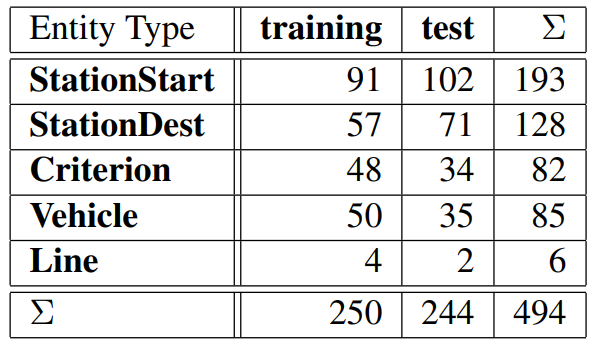
\includegraphics[width=10cm]{images/comparisonimg/1.png}
    \caption{Các loại thực thể trong kho ngữ liệu chatbot}
    \label{fig:comparisonimg-1}
\end{figure}

StackExchange Corpus

\begin{itemize}
    \item[--] Đối với bộ dữ liệu StackExchange, tác giả chọn ra những câu hỏi có đánh giá cao nhất và nhiều lượt xem nhất từ 2 nền tảng ask ubuntu và web applications,  bởi vì chúng có khả năng là có chất lượng tốt hơn các câu hỏi ít phổ biến hơn.
        \item[--]Bộ dữ liệu thu được tổng cộng là 290 câu hỏi, 100 câu từ web applications và 190 câu từ ask ubuntu.
        \item[--]Ý định và thực thể cũng được gán nhãn thủ công:
        \begin{itemize}
            \item[+]Đối với ask ubuntu, những ý định có thể là “Make Update”, “Setup Printer”, “Shutdown Computer”, and “Software Recommendation”. Những entity có thể có là : “SoftwareName”, “Printer”, and “UbuntuVersion”.
            \item[+] Đối với web applications, những ý định có thể có là “Change Password”, “Delete Account”, “Download Video”, “Export Data”, “Filter Spam”, “Find Alternative”, and “Sync Accounts”. Những entity có thể có là “WebService”, “OperatingSystem” and “Browser”.
        \end{itemize}
    \item[--] Sau khi gán nhãn và chọn lọc, bộ dữ liệu cuối cùng bao gồm 251 câu, trong đó 162 câu thuộc ask ubuntu và 89 câu thuộc web application.
    \item[--] Dữ liệu cũng được chia thành dữ liệu huấn luyện và dữ liệu kiểm thử như bảng sau:
\end{itemize}

\begin{figure}[H]
    \centering
    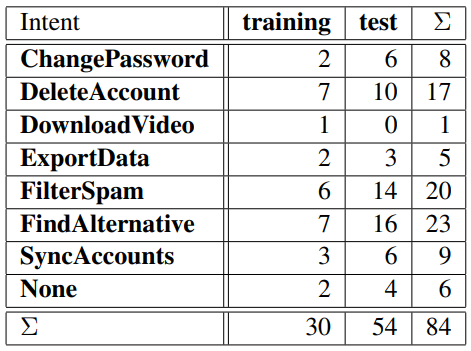
\includegraphics[width=10cm]{images/comparisonimg/webappdatasets.png}
    \caption{Bộ dữ liệu web applications}
    \label{fig:comparisonimg-webappdatasets}
\end{figure}

\begin{figure}[H]
    \centering
    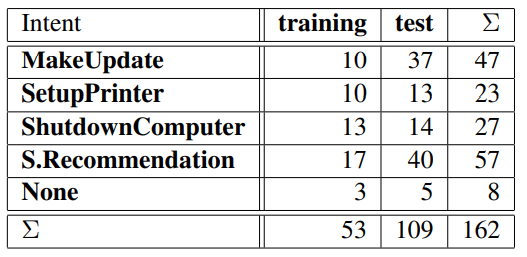
\includegraphics[width=10cm]{images/comparisonimg/askubuntudatasets.png}
    \caption{Bộ dữ liệu ask ubuntu}
    \label{fig:comparisonimg-askubuntudatasets}
\end{figure}

\begin{figure}[H]
    \centering
    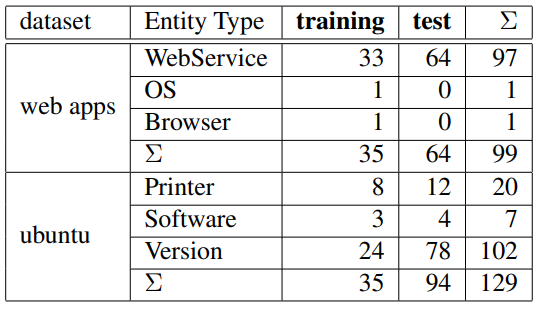
\includegraphics[width=10cm]{images/comparisonimg/entityTypesStackExchange.png}
    \caption{Các loại thực thể trong bộ ngữ liệu StackExchange}
    \label{fig:comparisonimg-entityTypesStackExchange}
\end{figure}

\textbf{Phần thí nghiệm}

\begin{itemize}
    \item[--] Tác giả huấn luyện mô hình trên các nền tảng LUIS, Watson Conversation, API.ai, và RASA. Tất cả đều dùng trên cùng một bộ dữ liệu.
        \item[--]Sau đó bộ dữ liệu kiểm thử đã được gửi đến các dịch vụ NLU để gán nhãn, đem gán nhãn được dự đoán bởi dịch vụ NLU so sánh với nhãn thực tế.
        \item[--]Để mà đánh giá kết quả, tác giả đã tính toán các độ đo precision và recall cũng như F-score cho từng intents, entity types, và từng bộ dữ liệu, cũng như kết quả tổng quát. Chúng ta sẽ nói rằng một dịch vụ tốt hơn dịch vụ kia nếu F-score của nó cao hơn.
\end{itemize}

\textbf{Đánh giá}

Kết quả thu được được mô tả dưới hình sau \ref{fig:comparisonimg-FscoresNLUServices}

\begin{figure}[H]
    \centering
    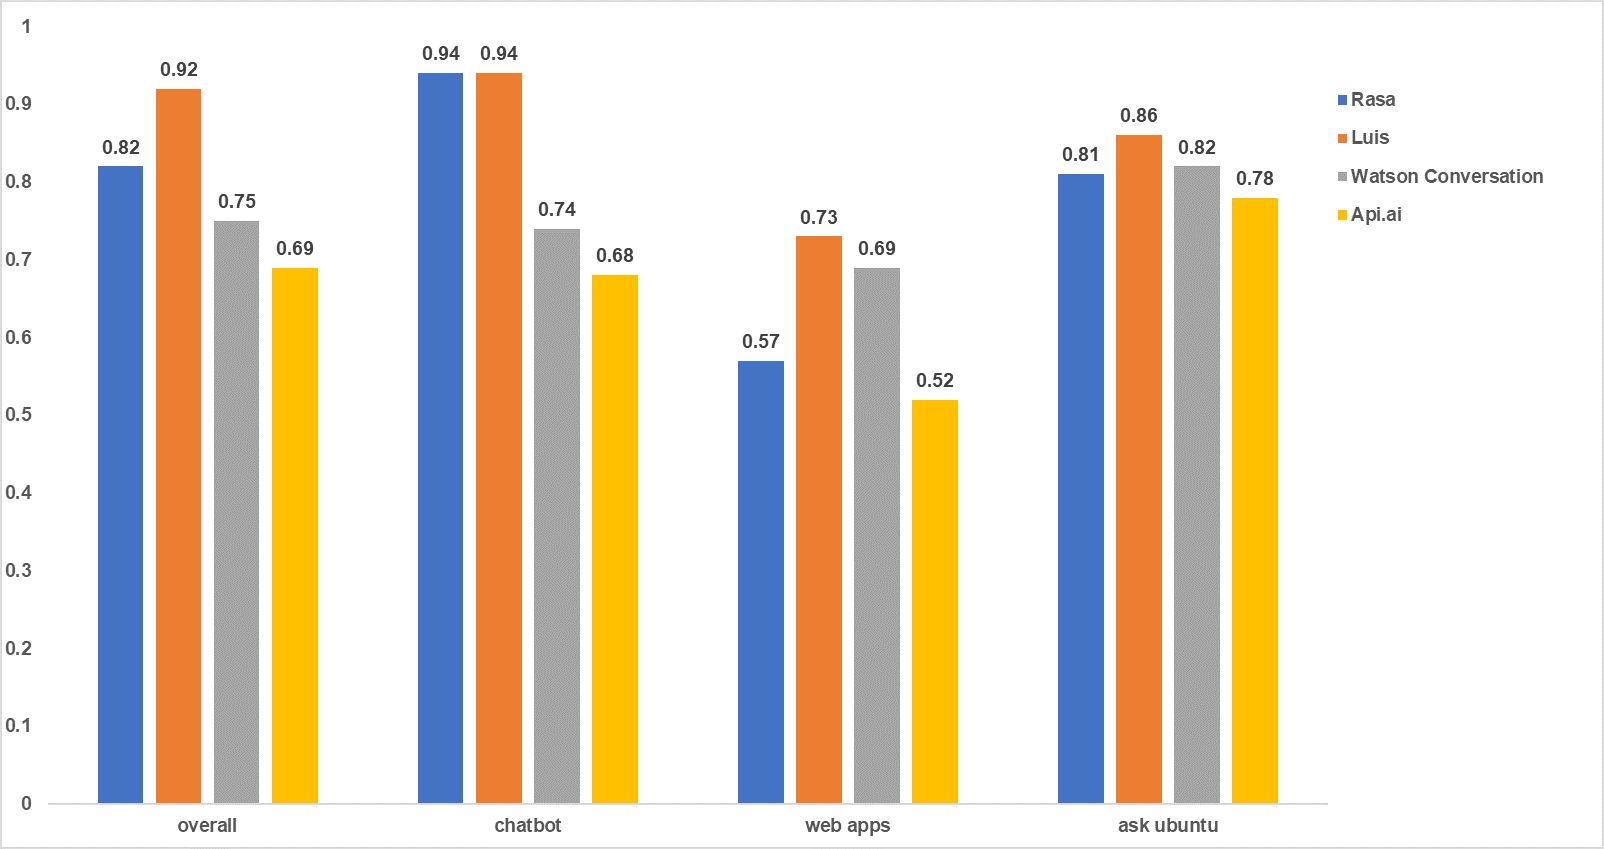
\includegraphics[width=10cm]{images/comparisonimg/FscoresNLUServices.png}
    \caption{F1-score của các dịch vụ NLU theo bộ ngữ liệu}
    \label{fig:comparisonimg-FscoresNLUServices}
\end{figure}

\begin{itemize}
    \item[--] Tổng quát LUIS có hiệu năng tốt nhất với F-score là 0.916, tiếp sau đó là là Rasa (0.821), Watson Conversation (0.752), and API.ai (0.687). Trên từng bộ dữ liệu: chatbot, web apps và ask ubuntu, LUIS cũng có hiệu năng cao nhất. Tương tự , API.ai có hiệu năng thấp nhất trên từng bộ dữ liệu, trong khi đó vị trí thứ 2 thay đổi giữa Watson và Rasa.
    \item[--] Dựa trên dữ liệu này, hiệu suất tốt nhất thuộc về sản phẩm thương mại LUIS, tuy nhiên phần mềm nguồn mở Rasa hiệu năng cao hơn các sản phẩm thương mại khác.
\end{itemize}

\textbf{II. Benchmarking Natural Language Understanding Services for building Conversational Agents}

Tương tự như bài báo trên, bài này cũng so sánh hiệu năng giữa các dịch vụ NLU bao gồm các sản phẩm thương mại: Dialogflow, LUIS và Watson, mã nguồn mở gồm Rasa.

\textbf{Dữ liệu: }

\begin{itemize}
    \item[--] Dữ liệu được thu từ người dùng thật thông qua Amazon Mechanical Turk (AMT). Các câu hỏi thuộc về cách mọi người tương tác với robot gia đình trong các tình huống được thiết kế trước, cụ thể là: alarm, audio, audiobook, calendar, cooking, datetime, email, game, general, IoT, lists, music, news, podcasts, general QA, radio, recommendations, social, food takeaway, transport, và weather.
    \item[--] Sau khi thu thập, gán nhãn và kiểm tra, dữ liệu cuối cùng thu được bao gồm 25716 câu nói, gồm 64 ý định và 54 loại thực thể.
\end{itemize}

\textbf{Thí nghiệm đánh giá}

Dữ liệu huấn luyện và kiểm thử
\begin{itemize}
    \item[--] Vì LUIS giới hạn kích thước dữ liệu huấn luyện, nên mỗi intent trong số 64 intent chọn ra ngẫu nhiên 190 câu nói. Một số intent có ít hơn 190 câu nói một chút.
    \item[--] Dữ liệu thu được là 11036 câu nói thuộc 64 ý định và 54 loại thực thể.
    \item[--] Đối với thử nghiệm đánh giá, tác giả sử dụng 10 fold cross-validation với 90\% dữ liệu huấn luyện và 10\% dữ liệu kiểm thử.
\end{itemize}

\textbf{Kết quả}

Dữ liệu từ hình \ref{fig:overallScores4IntentandEntity} cho thấy điểm trung bình cho phân lớp ý định và thực thể thông qua 10-fold cross validation.

Dữ liệu hình \ref{fig:combinedOverallScores} cho thấy điểm F-score trung bình cho mỗi nền tảng.

\begin{figure}[H]
    \centering
    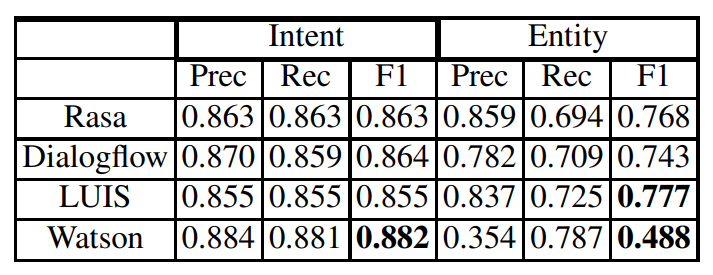
\includegraphics[width=10cm]{images/comparisonimg/overallScores4IntentandEntity.png}
    \caption{Các chỉ số của Intent và Entity}
    \label{fig:overallScores4IntentandEntity}
\end{figure}

\begin{figure}[H]
    \centering
    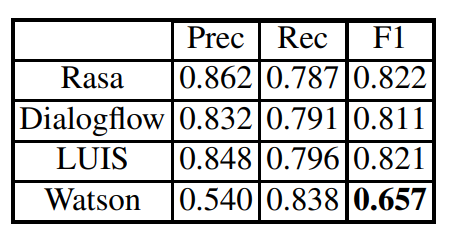
\includegraphics[width=10cm]{images/comparisonimg/combinedOverallScores.png}
    \caption{Điểm trung bình của cả Intent và Entity}
    \label{fig:combinedOverallScores}
\end{figure}

\begin{itemize}
    \item[--] Dựa vào hình \ref{fig:overallScores4IntentandEntity}, đối với intent, không có sự khác biệt lớn nào giữa Dialogflow, LUIS và Rasa. F1-score của Watson (0.882) tương đối cao hơn so với các nền tảng khác. Tuy nhiên đối với nhận diện thực thể, Watson có F1-score thấp do Precision rất thấp.
    \item[--] Hình \ref{fig:combinedOverallScores} chỉ ra rằng tất cả các dịch vụ có F1-score tương đương nhau ngoại trừ Watson có điểm thấp hơn đáng kể.
    \item[--] Trong bài so sánh này, ta thấy hiệu năng của Watson thấp nhất với F1-score là 0.657. Những nền tảng còn lại là Dialogflow, LUIS và RASA có hiệu năng tương đối cao, trong đó nền tảng mã nguồn mở Rasa có hiệu năng tốt nhất (0.822)
\end{itemize}

\textbf{III. Snips Voice Platform: an embedded Spoken Language Understanding system for private-by-design voice interfaces}

\begin{itemize}
    \item[--] Thử nghiệm này được thực hiện giống với phương pháp của bài báo đã được xuất bản trước đó. Evaluating Natural Language Understanding Services for Conversational Question Answering Systems. So sánh hiệu năng giữa các dịch vụ NLU khác nhau: một số giải pháp dựa trên đám mây phổ biến (Microsoft’s Luis, IBM Watson, API.AI nay là Dialogflow của Google) và nền tảng mã nguồn mở Rasa NLU.
    \item[--] Để biết kết quả thô, xem ở \url{https://github.com/sonos/nlu-benchmark}. Chỉ số chính được sử dụng trong điểm chuẩn này là F1-score trung bình của phân loại ý định và các thực thể.
\end{itemize}

\textbf{Dữ liệu}
\begin{itemize}
    \item[--] Dữ liệu bao gồm ba kho tài liệu. Hai trong đó được trích xuất từ StackExchange, một từ chatbot Telegram. Kết quả được trình bày trong hình \ref{fig:benchmark2017and2018}. Hình \ref{fig:averageF1-scores} trình bày trung bình kết quả trên ba kho tài liệu, tương ứng với phần tổng thể của hình \ref{fig:benchmark2017and2018}. Rasa được xem xét trên cả ba phần backend có thể có (Spacy, SKLearn + MITIE, MITIE). Tuy nhiên vì lý do thời gian huấn luyện, chỉ có Spacy được chạy trên cả 3 bộ dữ liệu.
    \item[--] Để công bằng, phiên bản mới nhất của Rasa NLU cũng được sử dụng. Kết quả cho thấy Snips NLU xếp hạng cao thứ hai về tổng thể.
\end{itemize}

\begin{figure}[H]
    \centering
    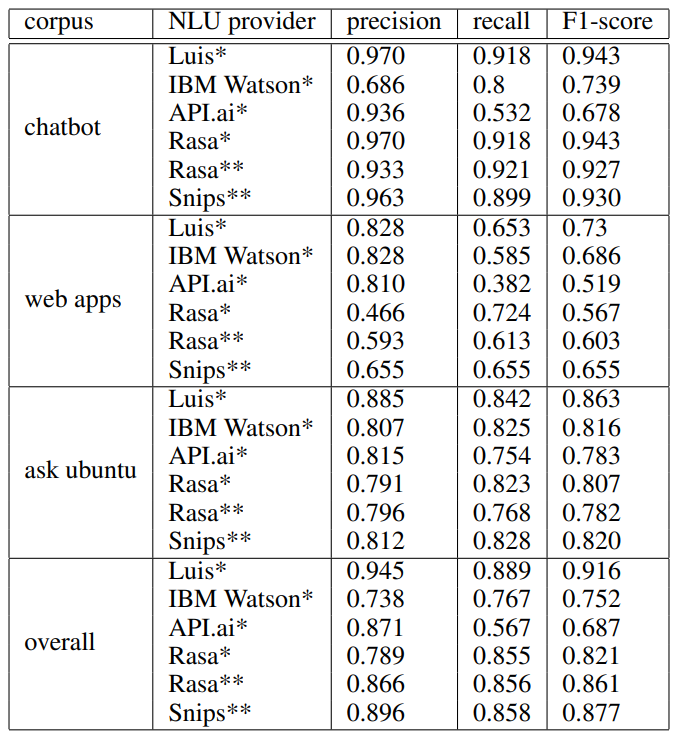
\includegraphics[width=10cm]{images/comparisonimg/benchmark2017and2018.png}
    \caption{Precision, recall và F1-score trên 3 bộ dữ liệu}
    \label{fig:benchmark2017and2018}
\end{figure}

\begin{figure}[H]
    \centering
    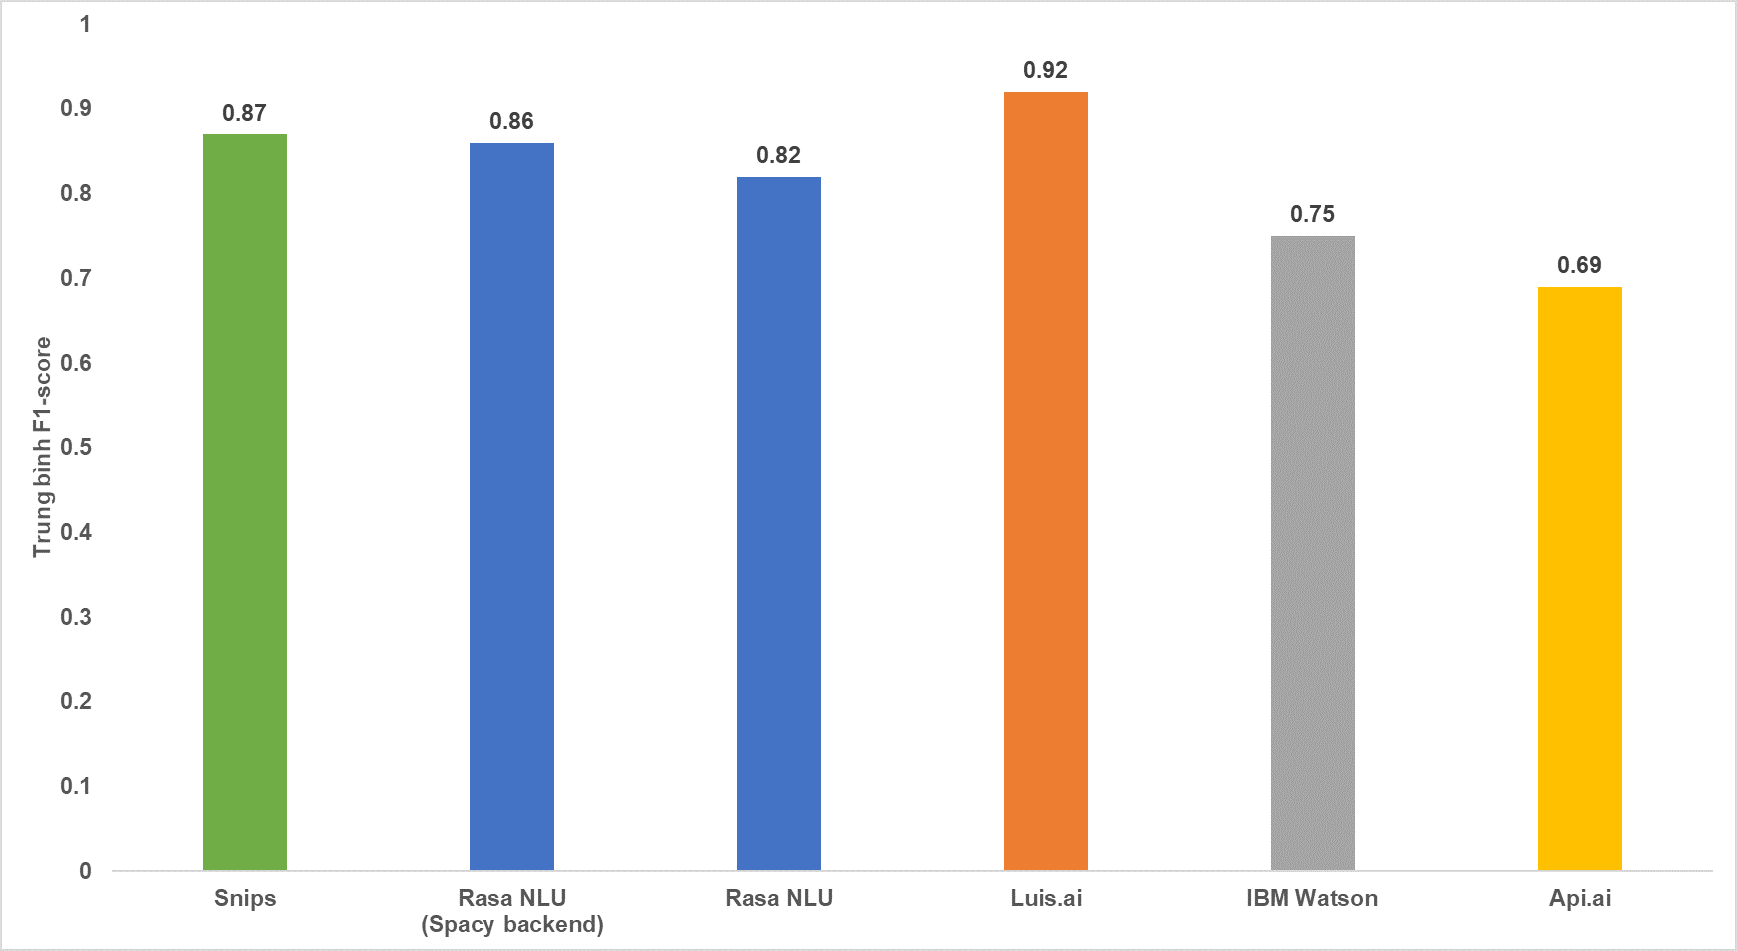
\includegraphics[width=10cm]{images/comparisonimg/averageF1-scores.png}
    \caption{Trung bình F1-score của Intent và Entity trên 3 bộ dữ liệu}
    \label{fig:averageF1-scores}
\end{figure}

\begin{itemize}
    \item[--] Dựa trên dữ liệu hình \ref{fig:benchmark2017and2018}, hiệu suất tốt nhất cũng thuộc về sản phẩm thương mại LUIS (F1-score 0.916), trong khi đó cả vị trí thứ 2 và thứ 3 đều thuộc về sản phẩm nguồn mở Snips (F1-score 0.877) và Rasa  (F1-score 0.861)
    \item[--] Trong bài này nhóm em quan tâm đến kết quả so sánh giữa Rasa với Snips (đều là 2 nền tảng nguồn mở). Khi cả 2 đều sử dụng phiên bản mới nhất và được đánh giá trên cùng một bộ dữ liệu, cả Rasa và Snips đều thể hiện hiệu năng tốt và không chênh lệch nhau nhiều. Tuy nhiên F1-score của Snips nhỉnh hơn một chút so với Rasa (F1-score của Snips là 0.877 và của Rasa là 0.861)
\end{itemize}

\subsection{Kết luận và lựa chọn nền tảng sử dụng}

\begin{itemize}
    \item[--] Dựa trên kết quả các bài báo mà nhóm tham khảo. Nhóm em rút ra được rằng giữa các nền tảng NLU khác nhau cho kết quả không giống nhau.
    \item[--] Các nền tảng nguồn mở vẫn có thể cạnh tranh được với các nền tảng thương mại. Mặc dù không có hiệu năng tốt nhất trên bảng so sánh, nhưng cả 2 nền tảng nguồn mở (Rasa và Snips) đều đứng ở vị trí thứ 2 và thứ 3 trong số 5 nền tảng được so sánh.
    \item[--] Nhóm em xem xét 2 nền tảng mã nguồn mở đó là Rasa và Snips để sử dụng trong nghiên cứu này. Nhóm quyết định sẽ chọn Snips NLU do nó có hiệu năng tốt hơn.
\end{itemize}